% MCR-GeoChem preprint. Generated by code/09_preprint.py from data/processed/stats.json and the release tables.
% Do not edit numbers here: edit the template and rebuild, so text and data cannot disagree.
\documentclass[aps,prd,twocolumn,superscriptaddress,nofootinbib,floatfix,10pt]{revtex4-2}
\usepackage[T1]{fontenc}
\usepackage{mathpazo}
\usepackage{amsmath,amssymb}
\usepackage{graphicx}
\usepackage{float}
\usepackage{dcolumn}
\usepackage{bm}
\usepackage{microtype}
\usepackage{xcolor}
\usepackage{xurl}
\usepackage{hyperref}
\hypersetup{colorlinks=false,linkbordercolor={1 0 0},citebordercolor={0 1 0},urlbordercolor={0 1 1},pdfborder={0 0 1}}
\usepackage{orcidlink}
\renewcommand{\arraystretch}{1.1}
<<DRAFTLINE>>

\begin{document}

\title{MCR-GeoChem: A harmonized, quality-flagged open compilation of whole-rock and mineral geochemistry for the 1.1~Ga Midcontinent Rift in Michigan, Minnesota, and Wisconsin}

<<AUTHORBLOCK>>

\begin{abstract}
Nickel, copper, cobalt, and the platinum-group metals are all on the final 2025 U.S. List of Critical Minerals, and the 1.1-billion-year-old Midcontinent Rift around Lake Superior hosts some of the largest domestic resources of them. The rock chemistry needed to study these systems is public but fragmented: it is spread across the U.S. Geological Survey (USGS) National Geochemical Database, project-level USGS data releases, the GEOROC compilation, and individual EarthChem datasets, each with its own units, method codes, and conventions for values below or above analytical limits. We present MCR-GeoChem v<<version>>, an open, versioned, reproducible compilation of <<n_samples>> Midcontinent Rift samples and <<n_det>> geochemical determinations (<<n_analytes>> analytes) from Michigan, Minnesota, and Wisconsin. Every value is converted to a common unit scheme (oxides in wt\%, trace elements in ppm, Au and platinum-group elements in ppb) while retaining its original form; censored values are decoded into an explicit qualifier and limit; <<n_methods>> source method codes are mapped to a common vocabulary of technique, digestion, and completeness; and each sample carries a rift-membership label tied to the USGS State Geologic Map Compilation. An open checker, \texttt{mcrqa}, adds value- and sample-level flags for below-detection results, uninformative detection limits, semi-quantitative and partial-digestion methods, unit errors, oxide-total problems, likely post-magmatic alteration, coordinate quality, and cross-source duplicates. The compilation shows that <<pct_semi>>\% of determinations derive from legacy semi-quantitative emission spectrography, that <<pt_unin>> of <<pt_n>> platinum results are below-detection values whose limits are too high to constrain the rock, and that <<n_ig_alt>> of <<n_ig_wr>> igneous whole-rock samples carry at least one alteration flag. The full pipeline rebuilds the release from public sources with identical results. The dataset, the method and detection-limit crosswalk, and the checker are released under open licenses to support critical-mineral research in the Lake Superior region.

\noindent\textbf{Keywords:} Midcontinent Rift, Keweenawan, Duluth Complex, critical minerals, platinum-group elements, geochemical data harmonization, detection limits, data quality
\end{abstract}

\maketitle

\section{Introduction}

Critical-mineral policy in the United States has turned attention back to old geological provinces whose resource potential was characterized decades ago with the analytical tools of the time. The final 2025 U.S. List of Critical Minerals, released by the U.S. Geological Survey (USGS) in November 2025, contains 60 commodities and includes nickel, cobalt, platinum, palladium, and, for the first time, copper~\cite{usgs2025list}. The 1.1~Ga Midcontinent Rift (MCR) of the Lake Superior region is one of the few places in the conterminous United States where all of these commodities occur in significant concentrations: magmatic Cu--Ni--platinum-group element (PGE) sulfide mineralization at the base of the Duluth Complex and in smaller conduit intrusions such as Eagle~\cite{ripley2014}, native copper in the Keweenaw Peninsula lavas and interflow conglomerates~\cite{brown2006}, and sediment-hosted stratiform copper in the Nonesuch Shale at White Pine and Copperwood~\cite{mauk1992}. The USGS Earth Mapping Resources Initiative (Earth MRI) funds new geologic, geophysical, and geochemical mapping in such regions~\cite{day2019}, and USGS Midcontinent Rift projects have recently released new drill-core geochemistry for the Duluth Complex~\cite{parks2025}.

Every one of these efforts begins with the same step: assembling the existing rock chemistry. That chemistry is public, but it is fragmented. The USGS National Geochemical Database (NGDB) now publishes 1.5 million samples analyzed between 1962 and 2023~\cite{granitto2026}; project data releases add newer analyses in their own formats~\cite{parks2025,woodruff2019,emri2025}; the GEOROC compilation, now being rebuilt as GEOROC 2.0~\cite{klocking2023b}, holds published analyses grouped by tectonic province and mineral~\cite{georoc_cfb,georoc_min}; and individual studies deposit their own tables in repositories such as the EarthChem Library~\cite{davis2022}. Each source uses its own units (element percent versus oxide weight percent, ppm versus ppb), its own codes for analytical methods, and its own conventions for values below a detection limit or above an upper limit. In the NGDB, for example, a value of $-0.5$ means ``less than 0.5,'' and a value of $10.11111$ means ``greater than 10''~\cite{granitto2026}. A user who joins these sources without decoding such conventions will silently treat a detection limit as a measured concentration, or an upper limit as a typing error.

These problems are well recognized in geochemistry. Community reviews call for machine-readable data with explicit units, methods, uncertainties, and provenance~\cite{klocking2023}, in line with the FAIR principles~\cite{wilkinson2016}. Statistical treatment of censored (below-detection) data is a mature field~\cite{helsel2012}, and the USGS ``best value'' approach provides a ranked choice among multiple determinations of the same element in one sample~\cite{granitto2019}. What has been missing for the MCR is a single open table that applies these practices across the major public sources, documents every decision, and flags rather than hides the quality problems that remain.

This paper describes MCR-GeoChem v<<version>>, built to fill that gap. Its contributions are:
(i) a harmonized compilation of <<n_samples>> samples and <<n_det>> determinations from <<n_sources_kept>> public sources, restricted to Midcontinent Rift rocks in Michigan, Minnesota, and Wisconsin by a documented membership rule;
(ii) a crosswalk that maps <<n_methods>> analytical-method codes to a common vocabulary, with a method-by-analyte detection-limit table;
(iii) an open quality-assurance checker, \texttt{mcrqa}, usable on any geochemistry table; and
(iv) a reproducible pipeline and provenance log that rebuild the release from the public sources.

The paper is organized as follows. Sec.~\ref{sec:geology} summarizes the geological setting and scope. Sec.~\ref{sec:sources} describes the sources. Sec.~\ref{sec:methods} sets out the harmonization, membership, crosswalk, best-value, and QA methods. Sec.~\ref{sec:results} describes the resulting dataset. Sec.~\ref{sec:validation} reports technical validation, Sec.~\ref{sec:usage} gives usage notes, Sec.~\ref{sec:limits} lists limitations, and Sec.~\ref{sec:conclusions} concludes.

\section{Geological setting and scope}
\label{sec:geology}

The Midcontinent Rift is a failed intracontinental rift that formed around 1.1~Ga and extends more than 2000~km from Kansas through the Lake Superior basin and south through Michigan~\cite{cannon1989,stein2014}. Seismic reflection profiling beneath Lake Superior imaged a very thick succession of rift volcanic and sedimentary rocks~\cite{cannon1989}, and it has been proposed that the rift was part of a larger plate-boundary system~\cite{stein2014}. Exposed rift rocks in the three study states comprise four broad groups~\cite{ojakangas2001}: (1) flood basalts and associated felsic volcanic rocks, including the Portage Lake Volcanics of the Keweenaw Peninsula, the Porcupine Volcanics and Powder Mill Group of Michigan and Wisconsin, the Chengwatana Volcanic Group, and the North Shore Volcanic Group of Minnesota; (2) large mafic intrusions, above all the Duluth Complex, together with the Beaver Bay Complex, the Mellen Complex, and numerous sills and dikes; (3) rift-basin sedimentary rocks of the Oronto Group (Copper Harbor Conglomerate, Nonesuch Shale, Freda Sandstone) and their equivalents; and (4) late- to post-rift sandstones of the Bayfield Group and Jacobsville Sandstone. Basalt geochemistry has been correlated across the rift to identify multiple mantle sources~\cite{nicholson1997}, and U--Pb geochronology shows that the Duluth Complex was emplaced during the main magmatic stage around 1.1~Ga~\cite{paces1993}, with much of its volume intruded rapidly~\cite{swansonhysell2021}.

The scope of v<<version>> is the rift as exposed or drilled in Michigan, Minnesota, and Wisconsin. Rift rocks in Ontario and the buried southern segment of the rift are outside the study area by design. Following the economic relevance of the province, all rift rocks are included, not only igneous rocks, and each sample carries a class label (rift igneous, rift sedimentary, or post-rift sedimentary) so users can select the subset they need.

\section{Data sources}
\label{sec:sources}

Table~\ref{tab:sources} lists the sources, their licenses, and the number of samples read, located in the study states, and retained. All are openly accessible. Sources S1, S2, S3, and S7 are USGS data releases in the U.S. public domain; S4--S6 are licensed CC~BY-SA~4.0.

<<TABLE_SOURCES>>

\textbf{S1, USGS NGDB 1962--2023.} The NGDB release of Granitto \textit{et al.}~\cite{granitto2026} (published January 2026) covers <<ngdb_total_us>> samples within U.S. boundaries. Since its November 2025 file update the ScienceBase bulk files (geodatabase, GeoPackage, Parquet) require a ScienceBase login; the same release is served by a public USGS ArcGIS feature service linked from the USGS Geochemical Data Portal. We queried its Rock, Mineral, and Geologic-material layers for \texttt{state IN ('MI','MN','WI')}, which returned <<s1_read>> samples. Each record carries one ``best value'' per species with its method code, and, where several determinations exist, a text field listing every value and method.

\textbf{S2, USGS Duluth Complex release.} Parks \textit{et al.}~\cite{parks2025} report <<s2_read>> drill-core and hand samples from the Duluth Complex and its footwall, with qualifier, numeric, and method columns for every element and a method dictionary.

\textbf{S3, USGS Earth MRI geochemistry v12.0.} The Earth MRI release~\cite{emri2025} contains <<s3_read>> rock samples in the three states. None are rift rocks (they are Archean, Paleoproterozoic, or Paleozoic), so S3 contributes no samples to v<<version>>; it remains in the pipeline so that later versions are screened automatically.

\textbf{S4, GEOROC Continental Flood Basalts, Midcontinent Rift System--Keweenawan.} The GEOROC precompiled file (generated 1 September 2026)~\cite{georoc_cfb} holds <<s4_read>> published whole-rock analyses from the whole rift, including Ontario; <<s4_in>> fall in the three study states.

\textbf{S5, GEOROC Minerals.} The 19 global GEOROC mineral files~\cite{georoc_min} (about 2.4 million analyses) were each downloaded, filtered to a box around the study region or to locations naming the rift, and discarded, leaving <<s5_read>> analyses for screening.

\textbf{S6, EarthChem Library dataset 1501.} Davis, Collins, and Rooney~\cite{davis2022} report XRF and LA-ICP-MS analyses of <<s6_read>> Portage Lake Volcanics samples with IGSN identifiers and a method metadata sheet.

\textbf{S7, USGS Duluth Complex basal contact.} Woodruff~\cite{woodruff2019} reports <<s7_read>> bedrock samples from three watersheds that cross the basal contact of the Duluth Complex, with an analytical-method and lower-limit table.

\textbf{Supporting sources.} Rift membership uses the USGS State Geologic Map Compilation (SGMC)~\cite{horton2017}; method definitions come from the method and parameter tables of the USGS Alaska Geochemical Database version 4 (AGDB4)~\cite{granitto2024}, which use the same method-code system as the NGDB; state assignment uses U.S. Census Bureau TIGER/Line 2023 state boundaries~\cite{tiger2023}.

\section{Methods}
\label{sec:methods}

\subsection{Acquisition and provenance}

A single script downloads every input and appends, for each file, the source identifier, file name, URL, access date, size in bytes, SHA-256 checksum, license, and full citation to a provenance log. Feature-service queries are paged and stored as JSON together with the query text and retrieval time. The provenance log is published with every release and rendered as a human-readable page with row counts.

\subsection{Data model}

The compilation has three linked tables. The \emph{samples} table has one row per sample (or per mineral analysis spot) with location, coordinate quality, sample type (whole rock, mineral grain, mineral separate), rock class, stratigraphy as given by the source, rift-membership class, and QA results. The \emph{long} table has one row per determination: sample identifier, analyte, harmonized value, unit, censoring qualifier, detection limit, method, a best-value indicator, and the original analyte name, unit, and value exactly as written in the source. The \emph{wide} table holds one row per sample with best values as columns, for convenience. Each sample has a permanent identifier of the form \texttt{MCRG-<source>-<source sample id>}.

\subsection{Unit harmonization}

Target units are oxide wt\% for major elements, loss on ignition (LOI), and volatiles; ppb for Au, Pt, Pd, Rh, Ru, Ir, Os, and Re; and ppm for all other elements. Sources that report major elements on an element basis (the USGS sources report Si, Ti, Al, Fe, Mn, Mg, Ca, Na, K, and P in percent) are converted to oxides with gravimetric factors,
\begin{equation}
c_{\mathrm{ox}} = f_{\mathrm{ox}}\, c_{\mathrm{el}}, \qquad f_{\mathrm{ox}} = \frac{M_{\mathrm{ox}}}{n\,M_{\mathrm{el}}},
\label{eq:oxide}
\end{equation}
where $M$ are molar masses and $n$ is the number of cation atoms per oxide formula unit. The factors used are listed in Table~\ref{tab:factors}. Total iron is expressed as Fe$_2$O$_3^{\mathrm{T}}$. FeO$^{\mathrm{T}}$ is converted with $f = 1.1113$, and where only Fe$_2$O$_3$ and FeO are reported,
\begin{equation}
\mathrm{Fe_2O_3^T} = \mathrm{Fe_2O_3} + 1.1113\,\mathrm{FeO},
\label{eq:fe}
\end{equation}
recorded as a derived value (<<n_derived_fe>> samples). In GEOROC files a lone \texttt{FE2O3} column (no FeO or FeO$^{\mathrm{T}}$ in the same sample) holds total iron in practice and is labeled Fe$_2$O$_3^{\mathrm{T}}$; the rule is recorded with the value. Unit changes between ppm, ppb, and wt\% use exact powers of ten. Non-chemical fields (density, pH, sample weights) are not carried.

<<TABLE_FACTORS>>

\subsection{Censored values}

Each determination is stored as a triple $(v, q, L)$ of value, qualifier, and limit:
\begin{equation}
(v,q,L) =
\begin{cases}
(x,\ \varnothing,\ \varnothing) & \text{measured},\\
(\varnothing,\ {<},\ L_{\mathrm{lo}}) & \text{below lower limit},\\
(\varnothing,\ {>},\ L_{\mathrm{hi}}) & \text{above upper limit}.
\end{cases}
\label{eq:censor}
\end{equation}
The NGDB qualified-value convention is decoded as follows: a negative number $-x$ becomes $({<}, x)$, and a number whose fractional part is $0.11111$ becomes $({>}, \lfloor x\rfloor)$~\cite{granitto2026}. Earth MRI uses the same negative-value convention~\cite{emri2025}. Text values such as \texttt{<0.5}, \texttt{>10000}, and \texttt{bdl} are parsed directly. The limit is converted to the target unit with the same factor as the value, so a censored Si result becomes a censored SiO$_2$ result with a converted limit. In the wide table, below-limit values are written as the negative of the limit, following the USGS convention, so that the file stays numeric.

\subsection{Rift membership}

A sample is retained only if (a) its coordinates fall in Michigan, Minnesota, or Wisconsin (TIGER/Line state polygons, including Great Lakes waters), and (b) a membership rule assigns it to the rift. We extracted all <<n_sgmc_units>> Mesoproterozoic SGMC map units in the three states and labeled each as rift igneous, rift sedimentary, post-rift sedimentary, or excluded (Table~\ref{tab:units}). Excluded units are the Wolf River batholith, Wausau and Stettin plutons (about 1.47--1.56~Ga, older than the rift) and the Minnesota unit of mafic intrusions of unknown age. For each sample, let $P$ be the text of its primary unit fields (stratigraphy, unit names), $S$ the text of secondary fields (deposit, project, locality), $A$ its geologic-age label, and $m$ the SGMC class at its location. With $R(\cdot)$ a match against a list of rift unit and locality names and $N(\cdot)$ a match against non-rift units and ages, the decision is
\begin{equation}
\mathrm{MCR} =
\begin{cases}
\text{yes (text)} & R(P) \wedge \neg N(P),\\
\text{no} & N(P) \vee N(A),\\
\text{yes (map)} & m \in \text{rift classes},\\
\text{yes (context)} & R(S) \wedge \neg N(S),\\
\text{no} & \text{otherwise},
\end{cases}
\label{eq:mcr}
\end{equation}
evaluated in that order. Membership classes are then refined: a sample whose source names a post-rift or rift-basin sedimentary unit takes that class, and an igneous rock on a sedimentary map polygon (a dike, or a mapping-scale effect) is labeled rift igneous. Each sample records how it was matched, so that users can drop the lower-confidence ``map'' and ``context'' matches. Every excluded sample is written to a separate table with its reason.

<<TABLE_UNITS>>

\subsection{Method crosswalk and detection limits}

Each source method code is mapped to a record giving the technique, the digestion or preparation, and an \emph{extent} class: total, near-total, partial, semi-quantitative, or unknown. For the NGDB the code grammar (technique prefix, digestion suffix, and a \texttt{\_P} partial marker) is combined with the AGDB4 method dictionary, which supplies descriptions, digestions, and references for <<n_codes_agdb>> of the <<n_codes_s1>> NGDB codes present; three rarely used codes are classified from the grammar alone. Codes from S2, S6, and S7 are mapped from each release's own method table. GEOROC precompiled files do not carry per-value methods and are marked ``not reported.'' The detection-limit table records, for each source, method, and analyte, the number of determinations, the number and share censored, the minimum and maximum limits actually reported with censored values, the documented lower limit of determination where available, and the USGS best-value rank of the method.

\subsection{Best values}

Where a sample has several determinations of one analyte, exactly one is marked as the best value. If the source designates a best value (NGDB, S2), it is kept. Otherwise determinations are ranked lexicographically by
\begin{equation}
\mathrm{rank} = \big(\mathbb{1}[\text{censored}],\ e,\ L\big),
\label{eq:best}
\end{equation}
where $e$ orders extents as total $<$ near-total $<$ unknown $<$ partial $<$ semi-quantitative, and $L$ is the detection limit. A measured value therefore wins over a censored one, a total digestion over a partial one, and a lower limit over a higher one.

\subsection{Quality-assurance checker}

The \texttt{mcrqa} package adds flags; it never changes values. Its thresholds are defaults with stated bases and can be overridden by a JSON file.

\textit{Value-level flags.} BDL marks $q={<}$; BDL\_UNINFORMATIVE marks censored values with $L > \tau_a$, where $\tau_a$ is an analyte-specific threshold near typical rock abundance (for example 10~ppb for Pt, Pd, and Au, and 50~ppm for Ni and Cu); ABOVE\_UPPER\_LIMIT marks $q={>}$; SEMI\_QUANTITATIVE, PARTIAL\_DIGESTION, and METHOD\_NOT\_REPORTED follow the crosswalk extent; IMPLAUSIBLE\_VALUE marks negative values (LOI excepted down to $-5$~wt\%), values above 100~wt\%, or above $10^6$~ppm; POSSIBLE\_UNIT\_ERROR marks whole-rock values above generous ceilings for unmineralized rock (for example 5000~ppm Ni or Cu, 2000~ppb Pt) unless the sample has $\geq 1$~wt\% S; and ZERO\_VALUE marks exact zeros.

\textit{Oxide totals.} When SiO$_2$, Al$_2$O$_3$, Fe$_2$O$_3^{\mathrm{T}}$, MgO, CaO, Na$_2$O, and K$_2$O are all measured and at least eight of the ten major oxides are present,
\begin{equation}
\Sigma = \sum_{i \in \mathrm{majors}} c_i + \mathrm{LOI},
\label{eq:total}
\end{equation}
with H$_2$O $+$ CO$_2$ substituted when LOI is missing. Totals outside 96--102.5~wt\% are flagged, except that low totals are not flagged when S $\geq 1$~wt\%, since sulfide-rich samples are not oxide-dominated. Requiring measured SiO$_2$ matters: HF-based digestions lose Si, and totals computed without it are meaningless. An igneous SiO$_2$ between 15 and 32~wt\% is flagged as a possible element-for-oxide error, because Si in a basalt is about 22--24~wt\%.

\textit{Alteration.} For igneous whole rocks, three indices are computed from best values. The Chemical Index of Alteration~\cite{nesbitt1982} is
\begin{equation}
\mathrm{CIA} = 100\,\frac{\mathrm{Al_2O_3}}{\mathrm{Al_2O_3} + \mathrm{CaO^*} + \mathrm{Na_2O} + \mathrm{K_2O}},
\label{eq:cia}
\end{equation}
in molar proportions, with $\mathrm{CaO^*} = \mathrm{CaO} - \tfrac{10}{3}\mathrm{P_2O_5} - \mathrm{CO_2}$ (molar, floored at zero) to remove apatite and calcite. The Ishikawa alteration index~\cite{ishikawa1976,large2001} is
\begin{equation}
\mathrm{AI} = 100\,\frac{\mathrm{MgO} + \mathrm{K_2O}}{\mathrm{MgO} + \mathrm{K_2O} + \mathrm{Na_2O} + \mathrm{CaO}},
\label{eq:ai}
\end{equation}
in wt\%. A sample is flagged ALTERED\_LOI if LOI $> 3$~wt\%, ALTERED\_CIA if CIA $> 60$, ALTERED\_AI if AI lies outside 20--65 (the least-altered field of the alteration box plot~\cite{large2001}), and ALTERED\_SOURCE if the source describes alteration. The summary indicator \texttt{altered\_likely} is true if any of these is set.

\textit{Coordinates.} Samples are flagged COORD\_MISSING, COORD\_APPROXIMATE (one decimal place, or the centroid of a GEOROC latitude--longitude box wider than 0.01$^\circ$), or COORD\_STATE\_MISMATCH.

\subsection{Cross-source duplicates}

The same physical sample can appear in more than one source, for example a Duluth Complex drill-core interval in both the NGDB and the 2025 USGS release. Two samples $j,k$ from different sources are linked if
\begin{equation}
\begin{split}
&\max(|\Delta\varphi|, |\Delta\lambda|) \le 0.005^\circ \ \wedge \\
&\big[\,\mathrm{ID}_j = \mathrm{ID}_k \ \vee\ (\delta_{\mathrm{SiO_2}} \le 1\% \wedge \delta_{\mathrm{MgO}} \le 1\%)\,\big],
\end{split}
\label{eq:dup}
\end{equation}
where $\varphi,\lambda$ are latitude and longitude, ID is the field or laboratory identifier normalized to upper-case alphanumerics, and $\delta$ is the relative difference. Linked samples are grouped by union--find. Duplicates are flagged and given a group identifier, not removed.

\subsection{Author corrections}

The pipeline changes no source value except by documented unit conversion and by corrections listed in a corrections file, each with the original value, the corrected value, the reason, the decision maker, and the date. One correction was applied in v<<version>>: USGS sample \texttt{MCRG-S2-1002826} is reported with Pd $=$ 123{,}000~ppb and Pt $=$ 123~ppb, a Pd/Pt ratio near 1000; the authors judged the Pd value a transcription error and normalized it to 123~ppb. The original value is kept in the long table, and the row carries the flag AUTHOR\_CORRECTED. We note that several other samples from the same deposit area (NorthMet, west pit) also show Pd far in excess of Pt, so Pd--Pt decoupling in Cu-rich sulfide cannot be excluded; confirmation has been requested from the data release authors, and users can recover the published value from \texttt{value\_source} or by setting aside the corrections file.

\subsection{Software and reproducibility}

The pipeline is a set of numbered Python scripts using pandas~\cite{mckinney2010}, GeoPandas, Shapely, and Matplotlib. A run-all script downloads the sources, builds and checks the tables, draws the figures, renders every number in the documentation from a statistics file written by the pipeline, and packages the release. The \texttt{mcrqa} checker is an installable package with a command-line interface for long-format tables and for ordinary wide spreadsheets, and with <<n_tests>> automated tests.

\section{Results}
\label{sec:results}

\subsection{Dataset composition}

MCR-GeoChem v<<version>> contains <<n_samples>> samples: <<n_mn>> in Minnesota, <<n_mi>> in Michigan, and <<n_wi>> in Wisconsin (Fig.~\ref{fig:map}). Of these, <<n_wr>> are whole-rock analyses and <<n_min>> are in-situ mineral analyses from GEOROC, dominated by zircon (<<n_zircon>>) with plagioclase, clinopyroxene, olivine, and sulfides. By rift class, <<n_ig>> samples are rift igneous, <<n_rsed>> rift sedimentary, and <<n_post>> post-rift sedimentary; by rock class, <<n_intr>> are intrusive and <<n_volc>> volcanic. Drill core supplies <<n_core>> samples and natural outcrop <<n_outcrop>>. The long table holds <<n_det>> determinations of <<n_analytes>> analytes, of which <<n_best>> are best values; <<pct_cens>>\% of best values are below detection. The NGDB supplies most samples (<<k_S1>>), followed by GEOROC rock analyses (<<k_S4>>), the 2025 USGS Duluth release (<<k_S2>>), GEOROC minerals (<<k_S5>>), EarthChem (<<k_S6>>), and the Woodruff release (<<k_S7>>).

Membership was decided by a named rift unit in the source for <<n_text>> samples (<<n_textmap>> of them also on a rift map unit), and by the map alone for <<n_map_only>> samples (Table~\ref{tab:units}). Of all samples read, <<n_excluded>> were excluded, most commonly because the source names a non-rift unit (for example Michigamme Slate, Biwabik Iron Formation, or Giants Range Granite) or a non-rift age, or because the coordinates fall outside the three states (most GEOROC rift samples outside the study area are in Ontario).

\begin{figure}[t]
\centering
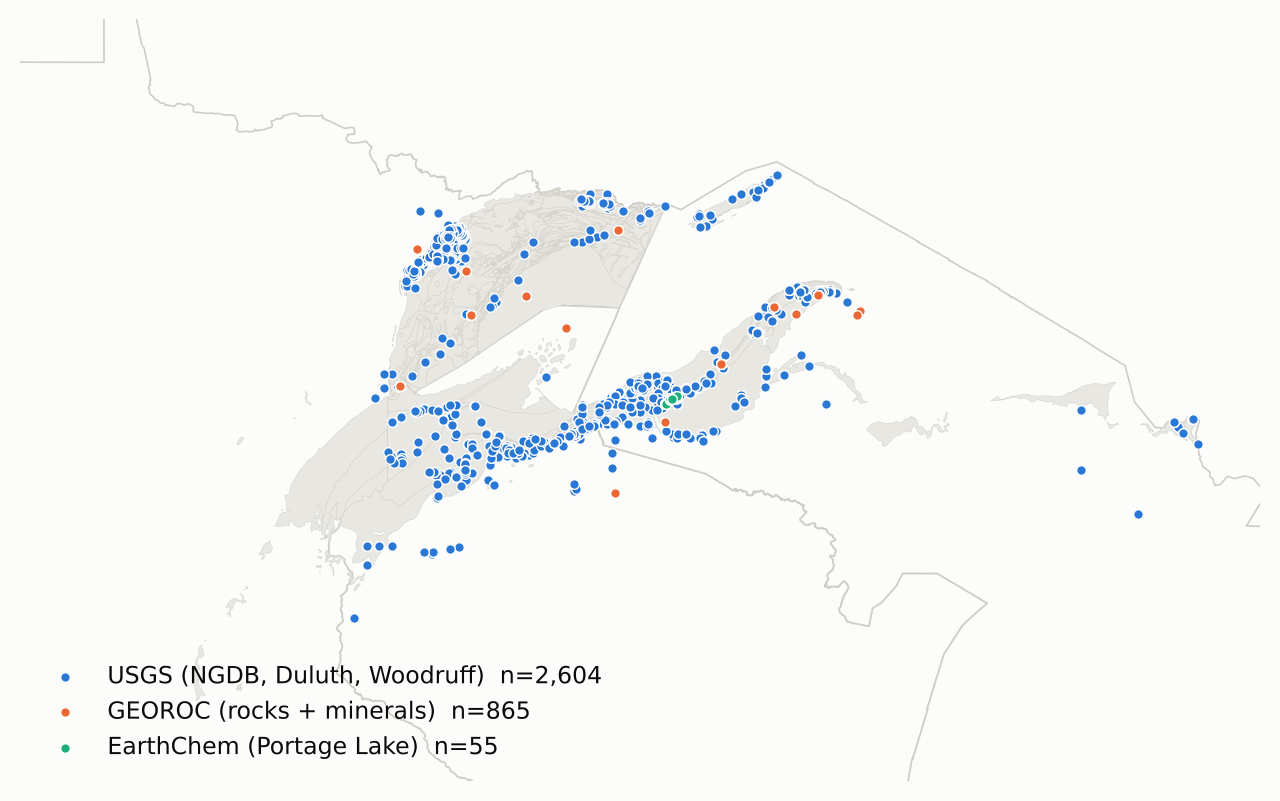
\includegraphics[width=\columnwidth]{../figures/paper_fig1_sample_map.png}
\caption{Locations of the <<n_samples>> MCR-GeoChem v<<version>> samples, grouped by source family, over the Mesoproterozoic rift map units of the USGS State Geologic Map Compilation used for membership (gray). State outlines are U.S. Census TIGER/Line 2023 boundaries, which include Great Lakes waters.}
\label{fig:map}
\end{figure}

\subsection{Analytical methods and detection limits}

After crosswalk harmonization the determinations fall into <<n_ext_total>> total, <<n_ext_near>> near-total, <<n_ext_partial>> partial, <<n_ext_semi>> semi-quantitative, and <<n_ext_unknown>> unknown-method records (Table~\ref{tab:extent}). The single largest technique family is DC-arc emission spectrography (Fig.~\ref{fig:methods}), the screening method of USGS geochemical surveys from the 1960s through the 1980s. Its results are reported in steps and carry high limits for precious metals. The ``not reported'' family consists entirely of GEOROC values.

<<TABLE_EXTENT>>

\begin{figure}[t]
\centering
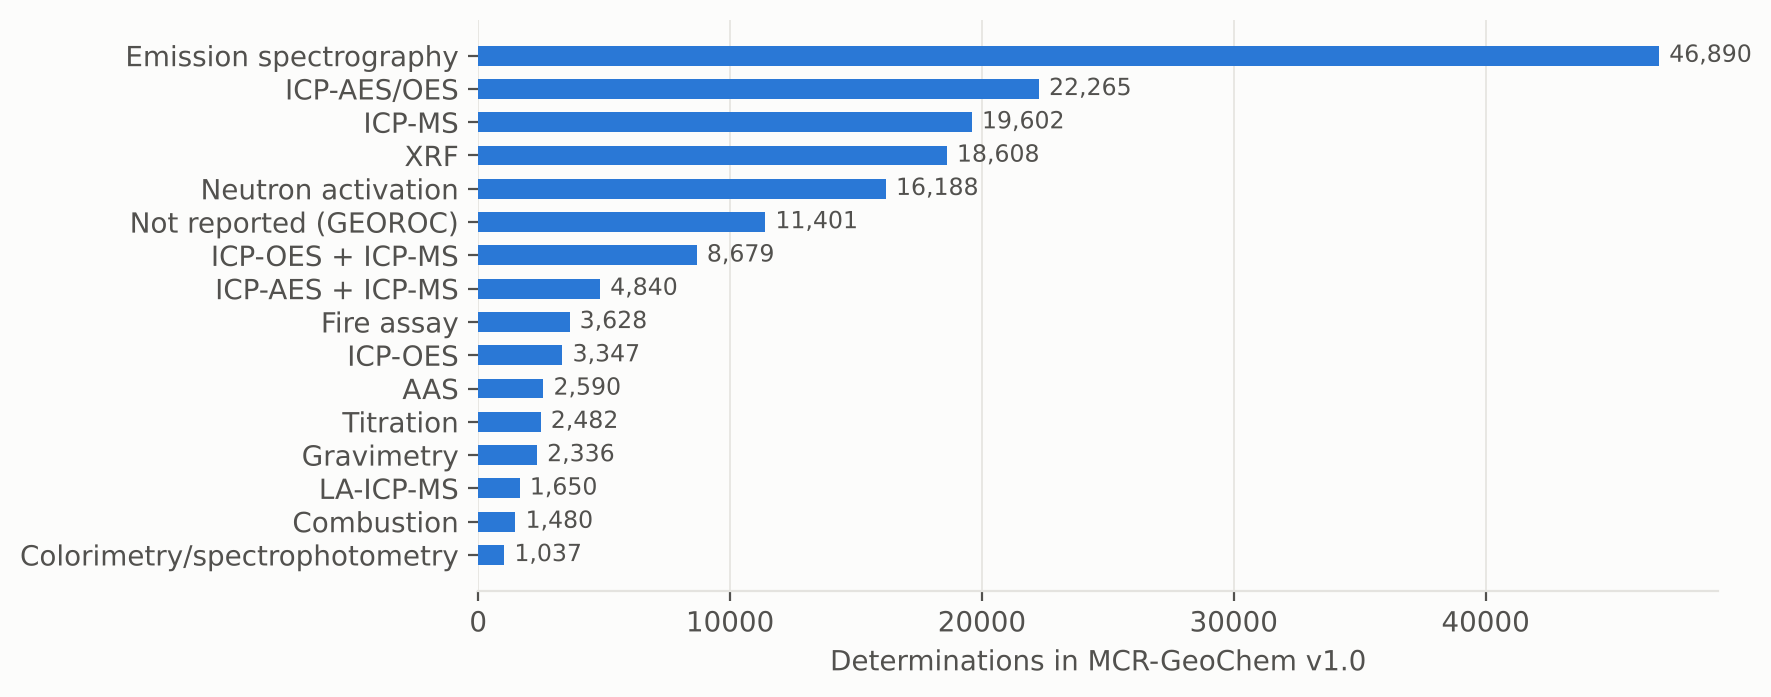
\includegraphics[width=\columnwidth]{../figures/paper_fig4_technique_families.png}
\caption{Determinations by analytical technique family after crosswalk harmonization (families with at least 500 determinations). The code-level mapping of all <<n_methods>> method codes is released as \texttt{method\_crosswalk.csv}.}
\label{fig:methods}
\end{figure}

\subsection{Critical metals}

Table~\ref{tab:metals} and Fig.~\ref{fig:metals} summarize best values for the critical base and precious metals. Nickel, copper, and cobalt are measured in <<pct_ni>>\%, <<pct_cu>>\%, and <<pct_co>>\% of the samples that report them, with median measured values of <<med_ni>>, <<med_cu>>, and <<med_co>>~ppm. The precious metals are a different story. Of <<pt_n>> samples with a platinum best value, only <<pt_det>> are measured; of the <<pt_bdl>> below-detection results, <<pt_unin>> have limits above 10~ppb, most from emission spectrography with limits of 1000--50{,}000~ppb. Palladium (<<pd_det>> of <<pd_n>> measured; <<pd_unin>> uninformative) and gold (<<au_det>> of <<au_n>>; <<au_unin>> uninformative) follow the same pattern. For these elements, a ``below detection'' entry in the legacy record says almost nothing about whether a rock is enriched, and treating it as zero, or as half the limit, would bias any regional assessment.

<<TABLE_METALS>>

\begin{figure}[t]
\centering
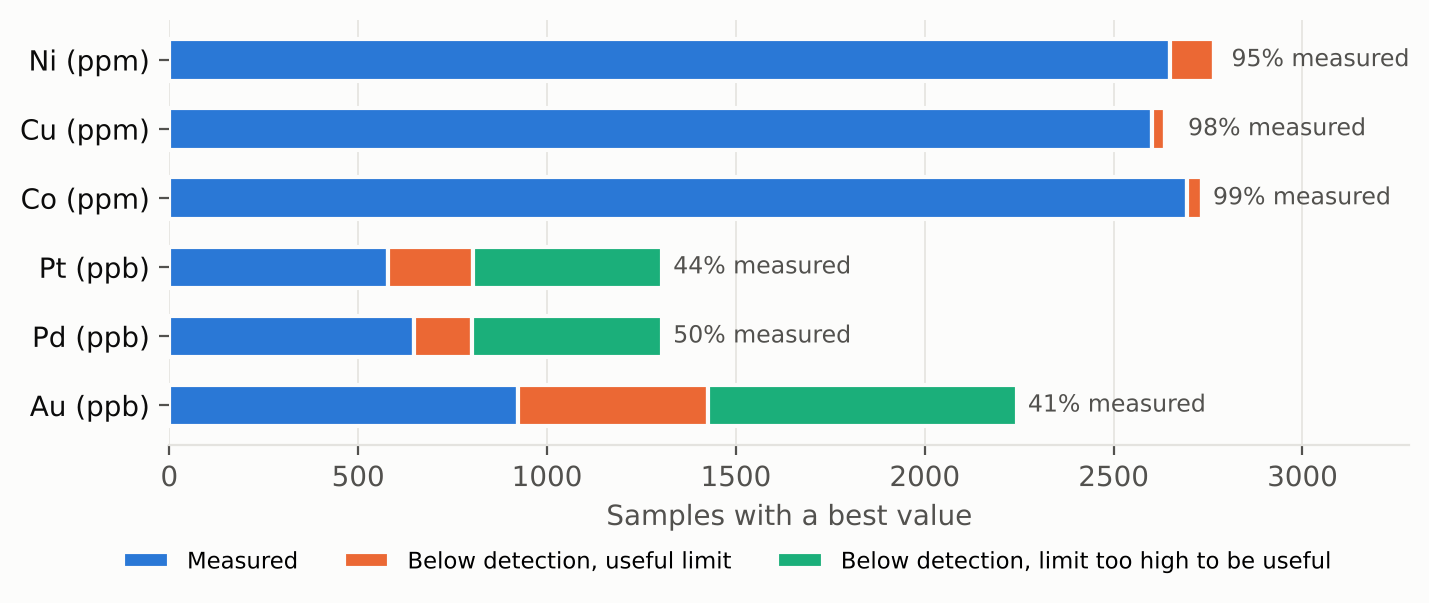
\includegraphics[width=\columnwidth]{../figures/paper_fig2_critical_metals_censoring.png}
\caption{Best values for critical metals, split into measured results, below-detection results with a useful limit, and below-detection results whose limit exceeds the \texttt{mcrqa} threshold (for example 10~ppb for Pt, Pd, and Au). Labels give the measured share.}
\label{fig:metals}
\end{figure}

\subsection{Quality-assurance outcomes}

Table~\ref{tab:flags} lists the flag counts and Fig.~\ref{fig:flags} the sample-level flags. At the value level, the most common flags are SEMI\_QUANTITATIVE (<<f_semi>>), BDL (<<f_bdl>>), BDL\_UNINFORMATIVE (<<f_unin>>), and METHOD\_NOT\_REPORTED (<<f_nomethod>>). Only <<f_unit>> values exceed the unit-error ceilings; inspection shows most are genuine ore samples (for example native-copper and chalcocite ore from the Nonesuch Shale) in which sulfur was not reported, so the sulfide exemption could not apply.

Of the <<n_tot>> samples with a computable oxide total, <<n_tot_ok>> fall within 96--102.5~wt\% (median <<tot_med>>~wt\%). At the sample level, <<n_coord_approx>> samples have approximate coordinates (nearly all from GEOROC), and <<n_dup_samples>> samples in <<n_dup_groups>> groups are probable cross-source duplicates. Among igneous whole rocks, <<n_ig_alt>> of <<n_ig_wr>> (<<pct_ig_alt>>\%) carry an alteration flag. The Ishikawa index fires most often (<<f_ai>>), followed by LOI (<<f_loi>>), source descriptions (<<f_src>>), and CIA (<<f_cia>>). Fig.~\ref{fig:tas} shows that flagged samples are concentrated at low alkali contents in mafic and ultramafic cumulates and at scattered positions off the main magmatic trend, as expected for samples whose alkalis were mobilized after crystallization.

<<TABLE_FLAGS>>

\begin{figure}[t]
\centering
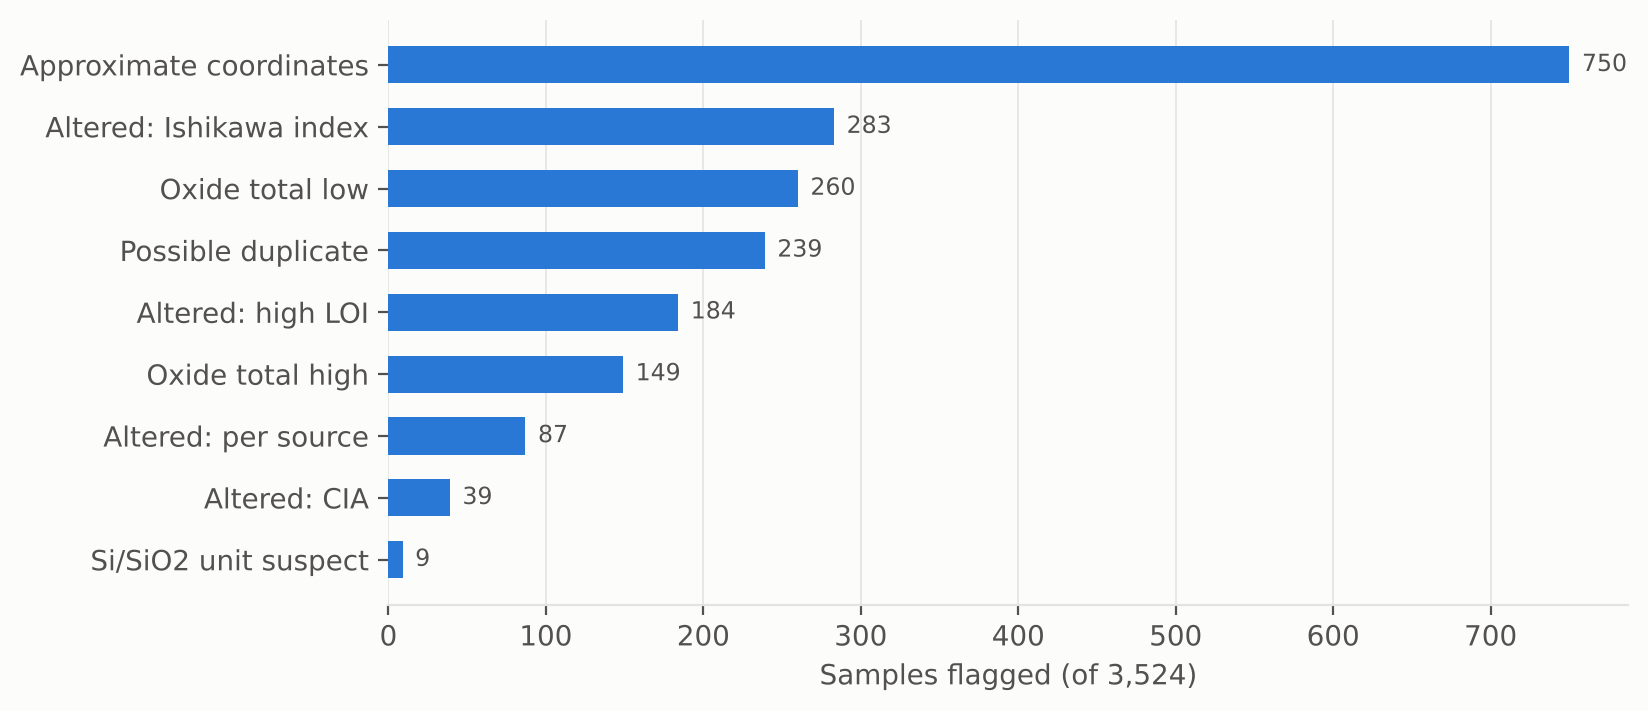
\includegraphics[width=\columnwidth]{../figures/paper_fig3_sample_qa_flags.png}
\caption{Sample-level flags from \texttt{mcrqa} for the <<n_samples>> samples. A sample can carry several flags.}
\label{fig:flags}
\end{figure}

\begin{figure}[t]
\centering
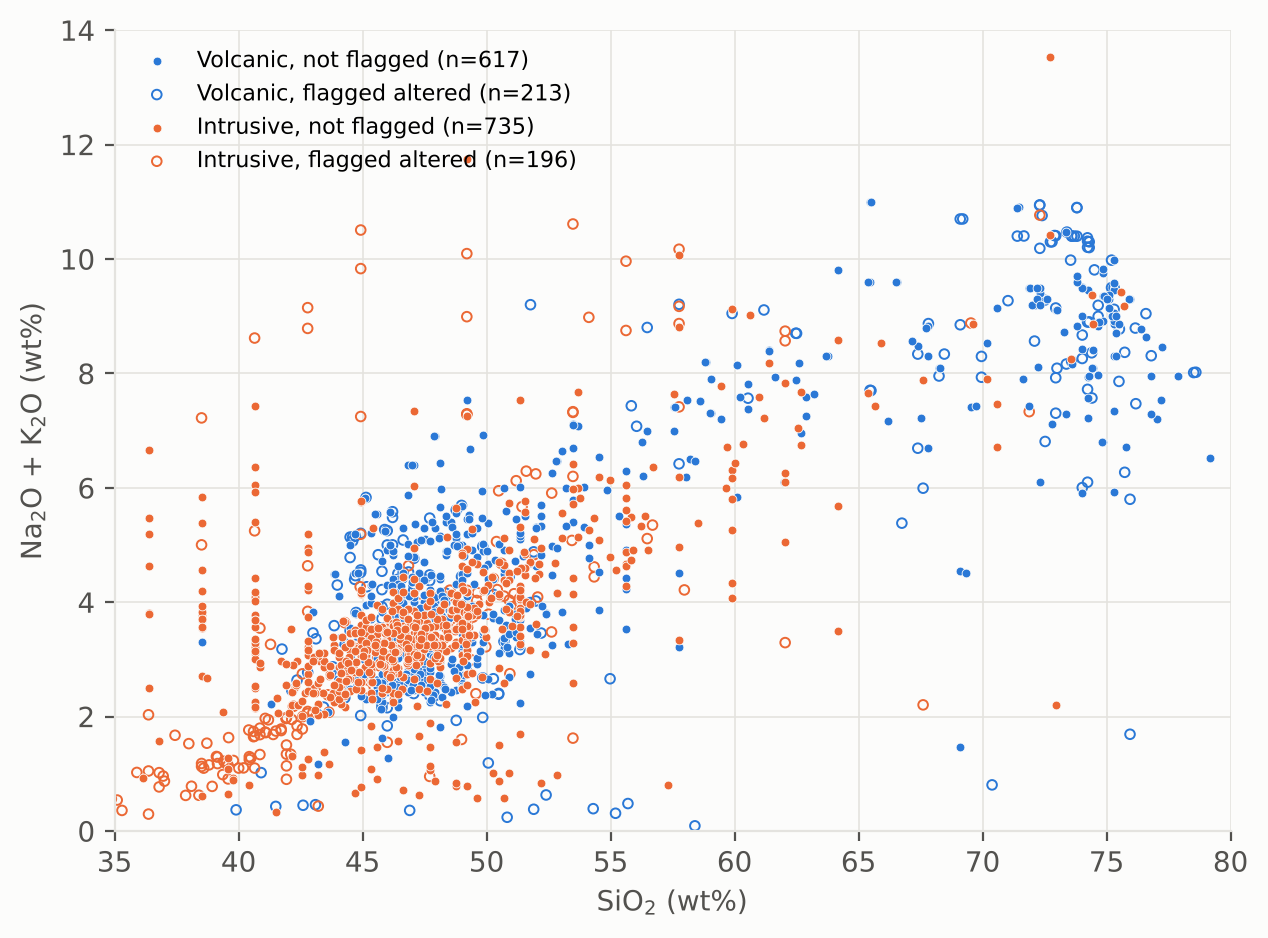
\includegraphics[width=\columnwidth]{../figures/paper_fig5_tas_alteration.png}
\caption{Total alkali versus silica for <<n_tas>> rift igneous whole rocks with measured SiO$_2$, Na$_2$O, and K$_2$O (best values). Open symbols carry at least one \texttt{mcrqa} alteration flag (LOI $>3$~wt\%, CIA $>60$, Ishikawa AI outside 20--65, or a source description of alteration).}
\label{fig:tas}
\end{figure}

\section{Technical validation}
\label{sec:validation}

\textbf{Reproducibility.} The complete pipeline was rerun in an empty folder, downloading every source again. The rerun reproduced every headline count (samples, determinations, best values, analytes, method codes, exclusions, state totals, alteration and duplicate counts, and critical-metal statistics) and produced byte-identical samples, wide, and crosswalk tables. The single author correction (Sec.~\ref{sec:methods}) is applied deterministically from the corrections file after harmonization, so it does not affect reproducibility.

\textbf{Spot checks against the sources.} Values chosen to include easy cases, hard cases, and extremes from every source were compared with the original records (Table~\ref{tab:spots}). All matched after the documented conversions; for example, NGDB Si $=$ 22.3\% becomes SiO$_2$ $=$ 47.71~wt\% by Eq.~(\ref{eq:oxide}), and an NGDB Pt value of $-30$~ppm is decoded as Pt $<$ 30{,}000~ppb. The same review flagged the Duluth palladium value corrected in Sec.~\ref{sec:methods}, whose Pd/Pt ratio near 1000 was implausible. A verification checklist distributed with the release adds five randomly selected best values (fixed random seed) and a review of excluded samples for independent checking by users.

<<TABLE_SPOTS>>

\textbf{Checker tests.} The <<n_tests>> unit tests of \texttt{mcrqa} cover the element-to-oxide and FeO$^{\mathrm{T}}$ conversions, PGE unit changes, decoding of the USGS negative and \texttt{.11111} conventions, text qualifiers, every value-level flag, oxide totals, the three alteration indices on fresh and altered basalt compositions, coordinate flags, duplicate grouping, and the wide-spreadsheet mode.

\textbf{Internal consistency.} Every determination links to exactly one sample and one crosswalk record; exactly one best value exists per sample and analyte; and every excluded sample has a reason. The median oxide total of <<tot_med>>~wt\% indicates that the unit conversions and the Fe$_2$O$_3^{\mathrm{T}}$ convention are applied consistently.

\section{Usage notes}
\label{sec:usage}

For regional statistics, keep one sample per \texttt{duplicate\_group}, use \texttt{is\_best\_value = True}, and decide explicitly how to treat censored values; methods for censored environmental data~\cite{helsel2012} apply directly. For precious metals, exclude BDL\_UNINFORMATIVE values or treat them as missing rather than as small concentrations. For igneous petrogenesis, filter on \texttt{altered\_likely = False}, on extent in \{total, near-total\}, and on \texttt{mcr\_match} in \{text, text+map\}. For mineral-potential work, retain semi-quantitative data as presence/absence screening evidence but do not mix them with quantitative data in averages. The checker can be applied to new data before merging: \texttt{mcrqa wide table.csv --id-col Sample --out qa/} reads USGS-style, GEOROC-style, or simple column headers and writes the flags and a summary.

\section{Limitations}
\label{sec:limits}

(1) State geological survey releases are not yet included; in October 2026 no machine-readable state chemistry table for rift rocks was found, and candidate reports are listed for v1.1. (2) The NGDB was taken from the public feature service, which lacks per-determination laboratory names and dates. (3) GEOROC precompiled files lack per-value methods and limits (<<f_nomethod>> values) and often give approximate coordinates. (4) <<pct_semi>>\% of determinations are semi-quantitative. (5) Rift membership is algorithmic; <<n_map_only>> samples rest on the 1:500{,}000-scale map alone, and contact-zone hornfels such as the Virginia Formation are excluded although they matter for sulfide genesis. (6) Alteration indices were designed for volcanic and fresh igneous rocks; cumulates and sulfide-bearing rocks can trip them. (7) Mineral chemistry is limited to <<n_min>> GEOROC analyses. (8) <<f_zero>> GEOROC values are exact zeros, kept and flagged. (9) NGDB depths often lack units and are not converted.

\section{Concluding remarks}
\label{sec:conclusions}

MCR-GeoChem v<<version>> provides, for the first time to our knowledge, an open, documented, and quality-flagged geochemistry table for the Midcontinent Rift in Michigan, Minnesota, and Wisconsin. It assembles <<n_samples>> samples and <<n_det>> determinations from six public sources, decodes their units and censoring conventions, maps <<n_methods>> method codes to a common vocabulary, and labels every sample's rift membership and quality. The compilation makes visible what is otherwise hidden when sources are merged naively: more than a quarter of the record is semi-quantitative; most below-detection precious-metal results cannot constrain the rocks; about one igneous sample in six shows signs of alteration; and the same drill core appears in more than one federal release. Because every flag is explicit and every decision documented, users can apply their own filters rather than inherit hidden ones. Version 1.1 will add state-survey tables, GEOROC methods from the GEOROC 2.0 interface, and additional mineral chemistry; the open checker can be applied to any of these additions, and to other provinces, before they are merged.

\section*{Data and code availability}

The dataset, the method and detection-limit crosswalk, the \texttt{mcrqa} checker, the pipeline, the provenance log, and the codebook are available at \url{https://github.com/bkdanso/mcr-geochem} (release v<<version>>) and are being archived on Zenodo, where each component receives its own DOI. Data are licensed CC~BY-SA~4.0, as required by the share-alike terms of the GEOROC and EarthChem inputs; code is MIT-licensed; documentation is CC~BY~4.0. Users should also cite the original sources~\cite{granitto2026,parks2025,emri2025,georoc_cfb,georoc_min,davis2022,woodruff2019}.

\section*{Author contributions}

<<CONTRIBUTIONS>>

\section*{Use of AI tools}

An AI assistant (Claude, Anthropic) was used to write pipeline code, documentation, and drafts of this manuscript under the authors' direction. The authors made all analytic decisions, verified the outputs against the sources, and take responsibility for the content.

\begin{acknowledgments}
We thank the U.S. Geological Survey for the National Geochemical Database and related data releases, the DIGIS team at the University of G\"ottingen for GEOROC, and the EarthChem Library and the data authors for making their data openly available.
\end{acknowledgments}

\clearpage
\onecolumngrid
<<APPENDIX>>

\clearpage
\twocolumngrid
<<BIBLIOGRAPHY>>

\end{document}
